\section{KNN}
\textbf{1.4.1 - Apply KNN and document the results. Explain the performance on the training and test-set}\\

To apply the KNN algorithm, the data was split into a 50\% training and 50\% test data, as requested. Furthermore labels for 0-9 were added for both training and test, this is to simply to be able to classify the data. The "class" library was used in order to make use of the KNN method. Table \ref{ref:resultsFor5K} shows the results for a K of 5, which was chosen at random, however even numbers were avoided in order to prevent a tie. The data applied for the KNN is based on one single person observations.

\begin{table}[H]
\centering
\begin{tabular}{|l|l|l|l|l|}
\hline
K & Accuracy & Observations  & Test duration & Training duration \\ \hline
5 & 96.35    & 4000          & 3.81 sec.     & Instance-based learning           \\ \hline
\end{tabular}
\caption{Results on applying KNN with K=5}
\label{ref:resultsFor5K}
\end{table}

KNN is a instance-based learner meaning that the algorithm does not learn anything. KNN stores everything in memory during the training time, which is fast. Test duration will on the other side take more time. The training and test was conducted on group4/member0, 100 DPI images.\\

\noindent
\textbf{1.4.2 - Performance of varying K: Show how performance ( speed and test recognition) changes with changing K}\\

Figure \ref{fig:accuracy30k} shows the varying of K compared with the accuracy. The larger K the smaller accuracy. One explanation could be due to the separation of the data. This experiment is based on 4000 observation based on one single person observations.

\begin{figure}[H]
\centering
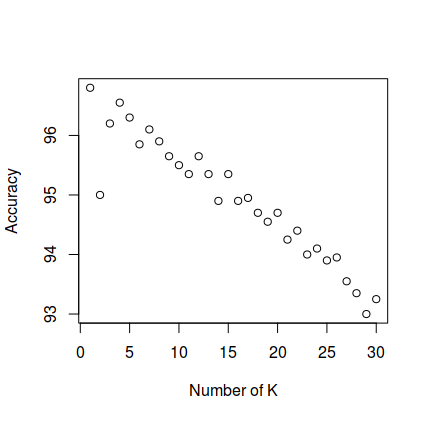
\includegraphics[scale=0.65]{Graphics/KNN/accuracy30K.png}
\caption{Accuracy with 30 different K's}
\label{fig:accuracy30k}
\end{figure}

According to figure \ref{fig:duration30k}, there does not seem to be any specific pattern to interpret. It was expected that the larger K is, the more time consuming it would be, but the graph does not show the expected result. 

\begin{figure}[H]
\centering
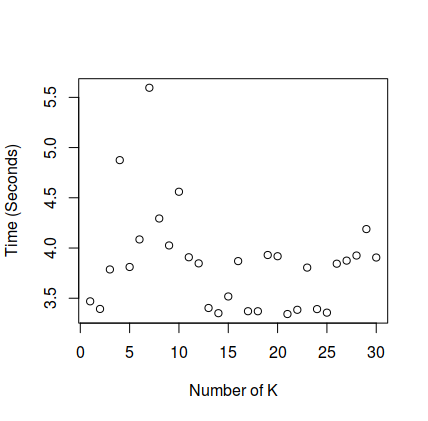
\includegraphics[scale=0.65]{Graphics/KNN/duration30K.png}
\caption{Duration of 30 different K's}
\label{fig:duration30k}
\end{figure}



\noindent
\textbf{1.4.3 - Cross validation: Perform a cross validation with a 90\% / 10\% split with 10 runs. Report mean and standard deviation of the performance.}\\

Running the cross validation results in a quite high mean accuracy and an acceptable standard deviation, as seen in table \ref{table:cvresult}. According to figure \ref{fig:cvplot}, 60\% of the results lies in the interval around the $97,25$ and $97,75$. $30\%$ of the results has a higher accuracy and only $10\%$ of the points lies beneath $97,25$. The data applied for the KNN is based on one single person observations.


\begin{table}[H]
\centering
\begin{tabular}{|l|l|l|l|l|}
\hline
K & Folds & Observations & Mean   & Standard deviation \\ \hline
5 & 10    & 4000         & 97.775 & 0.5583955          \\ \hline
\end{tabular}
\caption{Results from k-fold cross validation}
\label{table:cvresult}
\end{table}



\begin{figure}[H]
\centering
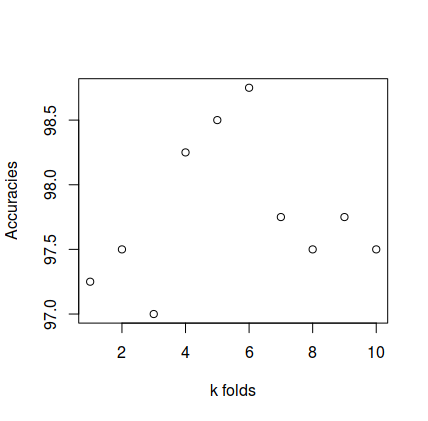
\includegraphics[scale=0.55]{Graphics/KNN/cvplot.png}
\caption{k-fold cross validation accuracies}
\label{fig:cvplot}
\end{figure}

\noindent
\textbf{1.4.4 - Preprocessing - apply smoothing functions}\\

By overriding the smooth function and running the smooth function with 6 different sigma, results in table \ref{table:result_over_smooth_on_image}. This experiment is based on 4000 observation based on one single person observations.  

\begin{table}[H]
\centering
\begin{tabular}{|l|l|l|l|l|}
\hline
K & Folds  & Sigma & Mean accuracy & Standard deviation \\ \hline
5 & 10     & 0.3   & 94.25         & 1.301708           \\ \hline
5 & 10     & 0.6   & 96.075        & 0.8253787          \\ \hline
5 & 10     & 1.0   & 97.425        & 0.9721825          \\ \hline
5 & 10     & 1.4   & 97.025        & 0.9313222          \\ \hline
5 & 10     & 1.8   & 96.4          & 0.7835106          \\ \hline
5 & 10     & 5.0   & 93.05         & 1.669997           \\ \hline
\end{tabular}
\caption{Result over smooth on image}
\label{table:result_over_smooth_on_image}
\end{table}

\noindent
\textbf{1.4.5 - Person independent KNN}\\

Table \ref{table:result_split_by_shuffle_data} shows the results after applying KNN on data from 10 groups with different members.

\begin{table}[H]
\centering
\begin{tabular}{|l|l|l|l|l|}
\hline
K & Total groups & Observations & Duration & Accuracy \\ 
\hline
5 & 10           & 80000                  & 26.61165 min   & 76.36       \\ \hline
\end{tabular}
\caption{Results of splitted shuffle data}
\label{table:result_split_by_shuffle_data}
\end{table}

Table \ref{table:person_independent} shows the results on applying KNN on person independent observations. The difference from table \ref{table:result_split_by_shuffle_data} is that data are ordered in the same way as the data is read from disk. The data are splitted in training and test where training consists of 5 groups and test consist of 5 groups. Within train and test data are shuffled.

\begin{table}[H]
\centering
\begin{tabular}{|l|l|l|l|l|}
\hline
K  & Total groups & Observations & Duration &  Accuracy \\ \hline
5  & 10           & 80000                  & 21 min   & 36.365        \\ 
\hline
\end{tabular}
\caption{Person independent}
\label{table:person_independent}
\end{table}

\noindent
\textbf{1.4.6 - Performance of sample size}\\

KNN are applied on different sizes of observation and different sizes of K. The results in table \ref{table:different_sizes} shows...

\begin{table}[H]
\centering
\begin{tabular}{|l|l|l|l|l|}
\hline
K  & Total groups & Observations & Duration &  Accuracy \\ \hline
5  & 10           & 80000                  & 21 min   & 36.365        \\ \hline
15 & 10           & 80000                  & 21 min   & 36.365        \\ \hline
25 & 10           & 80000                  & 21 min   & 36.365        \\ \hline
5  & 10           & 40000                  & 21 min   & 36.365        \\ \hline
15 & 10           & 40000                  & 21 min   & 36.365        \\ \hline
25 & 10           & 40000                  & 21 min   & 36.365        \\ \hline
\end{tabular}
\caption{Results on different K's and different sample sizes}
\label{table:different_sizes}
\end{table}